\documentclass{tccv}
\usepackage[hmargin=0.2cm,vmargin=0cm]{geometry}
\usepackage{amsfonts} 								% for the \checkmark command 
\usepackage[framemethod=TikZ]{mdframed}						% For box around text

\usepackage[overlay,absolute]{textpos}
\setlength{\TPHorizModule}{1cm}
\setlength{\TPVertModule}{1cm}

\usepackage{fontspec}




\mdfsetup{
   middlelinecolor=mybluegrey,
   middlelinewidth=2pt,
   backgroundcolor=white!0,
   roundcorner=10pt,
   skipabove=0,
   fontcolor=black,
}

\fontdir[fonts/]
\colorlet{awesome}{awesome-skyblue}


\begin{document}
%%%%%%%%%%%%%%%%%%%%%%%%%%%%%%%%%%%%%%%%%%%%%%%%%%%%%%%%%%%%%%%%%%%%%%%%%%%%%%%%%%%%%%%%%%%%%%%%%%%%%%%%%%%%%%%%%%%%


\begin{textblock}{6.5}(0.5,0.5)
\personal
    []
    {16 Rue Chicogné, 35000 Rennes}
    {+33 07 83 88 33 32}
    {r.sanhuezarepetto@gmail.com}
\end{textblock}

\begin{textblock}{10}(8.0,1)
      \headerfirstnamestyle{Roc\'io}   \headerlastnamestyle{Sanhueza}
\end{textblock}

\begin{textblock}{21}(17.5,0.5)
		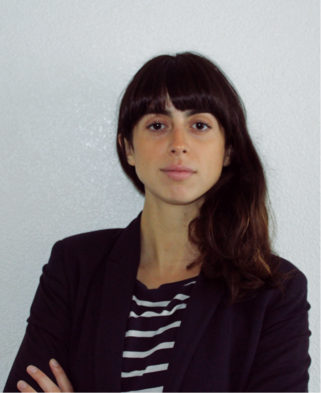
\includegraphics[width=3cm]{../Figure/Rocio3.png}
\end{textblock}  









\begin{textblock}{7}(0.5,4)
\begin{mdframed}

\section{Education}
\begin{yearlist}

\item[Master 1 Science politique]{2015 -- 2016}
     {Université de Rennes 1}
     {Enseignements suivis: pensée politique contemporaine, 
     régimes contemporaines, sociologie de la communication, pensée sociologique, 
     Approches de l'Union Européen, Grand dossiers de l'administration.}


  

\item[Diplôme en Communication sociale et journalisme (Bac+5)]{2008 -- 2013}
     {Universidad de Santiago de Chile}
     {Mention très bien
      Spécialité politique
      }

     
\item[Échange universitaire -- journalisme]{2011 -- 2011}
     {Universidade Estadual Paulista }
     {Enseignements suivis: réalité socio - économique et politique brésilienne. \\
     Langue portugaise: littérature, sémiotique, stratégies de communication publique}


\end{yearlist}
\end{mdframed}


\begin{mdframed}
\section{Compétences linguistiques}

\begin{factlist}
\item{Espagnol} {Langue maternelle}	
\item{Français} {Courant}	
\item{Anglais}  {Niveau B2}	
\item{Portugais}{Niveau B2}
\end{factlist}

\section{Logiciels}
\descriptionstyle{
Environnement PC et Linux,
Pack office et libre office,
Adobe Photoshop, Premiere, \\
%Python, 
Gimp,
HTML5,
\LaTeX.
}


\section{Aptitudes}
\descriptionstyle{
  Aisance communicationnelle et relationnelle. \\
  Disciplinée et organisée. \\
  Esprit d'équipe. \\  
}



%%%%%%%%%%%%%%%%%%%%%%%%%%%%%%%%%%%%%%%%%%%%%%%%%%%%%%%%%%%%%%%%%%%%%%%%%%%%%%%%%%%%%%%%%%%%%%%%%%%%%%%%%%%%%%%%%%%%%%%%%%%%%%%%%%%%%%%%%%
%&
\end{mdframed}
\end{textblock}


\mdfsetup{middlelinecolor=white!0}

\begin{textblock}{13}(7.7,4)
\begin{mdframed}
\section{Experience Professionnelle}


\begin{eventlist}
\item{Avril 2014 -- Mars 2015}
     {Sénat du Chili}
     {Conseillère en communication et attachée de presse}
     \descriptionstyle{ 
     Contexte : Cabinet politique du sénateur Felipe Harboe. \\ 
     Missions : 
     }  

  \setlength{\parskip}{-10pt}
    \begin{itemize}
      \setlength\itemsep{-3pt} 
      \cvitem[\checkmark]  \descriptionstyle{ Mise en œuvre des actions de communication et des relations avec la presse                     }
      \cvitem[\checkmark]  \descriptionstyle{ Rédaction des articles, communiqués et dossiers de presse. Gestion et supervision des interviews avec les médias      }
      \cvitem[\checkmark]  \descriptionstyle{ Organisation des conférences de presse                                                                                               }
      \cvitem[\checkmark]  \descriptionstyle{ Administration de réseaux sociaux                                                    }
    \end{itemize}     
     \descriptionstyle{ 
    Résultat : Présence constante dans la presse nationale et régionale  \\
               Entre 600 et 1100 visites quotidiennes au site web personnel
      }
               
\item{Mai 2013 -- Déc. 2014}
     {Aluro 35, Santiago, Chili}
     {Productrice générale}
     
          \descriptionstyle{ 
Contexte : Maison de production indépendante Aluro 35 doit produire le programme culturel de télévision La Bicicleta qui se transmit par la chaîne 13C \\
Missions :
     }  
     
    \begin{itemize}
      \setlength\itemsep{-3pt} 
      \cvitem[\checkmark] \descriptionstyle{ Gestion des rapports avec la chaîne et négociation de budgets                          }
      \cvitem[\checkmark] \descriptionstyle{ Préparation du lieu de tournage, mobilisation, catering et interviewés de chaque chapitre. Aide à la préparation du contenu des entretiens   }
      \cvitem[\checkmark] \descriptionstyle{ Administration de réseaux sociaux et animation de communautés (Facebook, Twitter, Instagram)                                                 }
      \cvitem[\checkmark] \descriptionstyle{ Création du dossier de presse pour les lancements du programme                                                   }

    \end{itemize}     
   \descriptionstyle{  
Résultats: Rénovation d'une deuxième saison avec une augmentation des sponsors.  \\
Important visibilité aux artistes ou associations culturels qui ont été interviewés \\
Gagnants d’un fond public du Conseil de Culture et Communication pour une troisième saison.  \\
     }
     
     
\item{Oct. 2013 -- Fév. 2014 }     
  {Agence de communication Más comunicaciones, Santiago, Chili}     
  {Journaliste}


\begin{itemize}
      \setlength\itemsep{-3pt} 
      \cvitem[\checkmark] \descriptionstyle{ Préparation d'articles pour les médias                                            }
      \cvitem[\checkmark] \descriptionstyle{ Création de dossiers de presse                                                     }
      \cvitem[\checkmark] \descriptionstyle{ Ciblage des journalistes spécialisés et amélioration de la basse de donnés.  }
\end{itemize}       



\item{Avril 2012 -- Avril 2013 }     
  {Killahue corporation, Santiago, Chili}     
  {Chargée de projet}

\begin{itemize}
      \setlength\itemsep{-3pt} 
      \cvitem[\checkmark]  \descriptionstyle{ Recherche des informations juridiques et environnementales des projets similaires                  }
      \cvitem[\checkmark]  \descriptionstyle{ Gestion et coordination des réunions, plus la préparation des matériaux visuel et écrit    }
      \cvitem[\checkmark]  \descriptionstyle{ Administration de réseaux sociaux                                                                                                            }
      \cvitem[\checkmark]  \descriptionstyle{ Formalisation et rédaction du travail réalisé et des décisions pris dans l’ensemble des réunions                                             }

\end{itemize}      

  
  
\iffalse
\item{Janv. 2012 -- Mars 2012 }     
  {Terra Networks, Santiago, Chili}     
  {Journaliste stagiaire – section économie}

\begin{itemize}
      \setlength\itemsep{0cm} 
      \cvitem[\checkmark] Rédaction des articles et notes d’économie national et internationale
      \cvitem[\checkmark] Traduction des nouvelles du portugais ou anglaise au espagnol
      \cvitem[\checkmark] Veille et mise à jour du site économique
      \cvitem[\checkmark] Réalisation des interviews et couverture médiatique des thèmes économiques nationaux

\end{itemize}        
\fi
   


\end{eventlist}


\end{mdframed}
\end{textblock}
\end{document}
